% !TEX root = ../main.tex

% Body section
\section{Asymptotic Normality and Efficiency of MLE}
The proofs for both the \emph{asymptotic normality of MLE} and the \emph{Cramer-Rao lowerbound} are well-documented in \cite{hogg2005introduction}, although some of the details and explanations are left out. In this section, we present both of these results following the main ideas in \cite{hogg2005introduction}, and fill in much of the left-out details. In particular, since the relevance of the regularity conditions that we have assumed in \cref{sec:notation} may not be immediately clear, we point out, in the subsequent sections, how each of them are essential to arriving at both the \emph{asymptotic normality of MLE} and the \emph{Cramer-Rao lowerbound}.
\subsection{Score Function and Fisher Information}
To begin, we define two functions of the derivative of the log-likelihood function. The \emph{score function} $\frac{\partial\log f(x;\theta)}{\partial\theta}$ is defined to be the derivative of the log-likelihood function of a single observation. And the \emph{Fisher information} is defined as
\begin{align}
I(\theta) = \bbE_{\theta}\left[ \left( \frac{\partial}{\partial\theta}\log f(X_1;\theta) \right)^2 \right]. \label{eqn:fisher}
\end{align}
These two quantities repeatedly come up in the proofs of both the \emph{asymptotic normality of MLE} and the \emph{Cramer-Rao lowerbound}. Using (R4) and (R5) from the regularity conditions, we can show the following properties of the score function and Fisher information through some simple algebraic manipulations.
\begin{lemma} \label{lem:2}
Under regularity conditions and using the notations set up in \cref{sec:notation}, we have
\begin{align*}
\bbE_\theta\left( \frac{\partial\log f(X_1;\theta)}{\partial \theta} \right) = 0, \text{ and }
I(\theta) = -\bbE_\theta\left[ \frac{\partial^2\log f(X_1;\theta)}{\partial \theta^2} \right] = \var_\theta\left( \frac{\partial\log f(X_1;\theta)}{\partial \theta} \right).
\end{align*}
\end{lemma}
\begin{proof}
We begin with differentiating both sides of $1 = \int_\bbR f(x;\theta) dx$.
\begin{align}
0 = \int_\bbR \frac{\partial}{\partial\theta} f(x;\theta)dx
= \int_\bbR \frac{\frac{\partial}{\partial\theta} f(x;\theta)}{f(x;\theta)}f(x;\theta) dx
= \int_\bbR \frac{\partial \log f(x;\theta)}{\partial\theta}f(x;\theta) dx 
= \bbE_\theta\left[ \frac{\partial \log f(x;\theta)}{\partial\theta} \right]. \label{eqn:trick_1}
\end{align}
Differentiating with respect to $\theta$ again, we get
\begin{align}
0 &= \frac{\partial}{\partial\theta}\int_\bbR \frac{\partial \log f(x;\theta)}{\partial\theta}f(x;\theta) dx\nonumber\\
&= \int_\bbR \frac{\partial^2 \log f(x;\theta)}{\partial\theta^2}f(x;\theta) dx + \int_\bbR \frac{\partial \log f(x;\theta)}{\partial\theta}\frac{\partial f(x;\theta)}{\partial\theta} dx\nonumber\\
&= \int_\bbR \frac{\partial^2 \log f(x;\theta)}{\partial\theta^2}f(x;\theta) dx + \int_\bbR \frac{\partial \log f(x;\theta)}{\partial\theta}\frac{\partial \log f(x;\theta)}{\partial\theta}f(x;\theta) dx \label{eqn:trick_2} \\
&= \bbE_\theta\left[ \frac{\partial^2 \log f(x;\theta)}{\partial\theta^2} \right] + \bbE_\theta\left[ \left(\frac{\partial \log f(x;\theta)}{\partial\theta}\right)^2 \right],\nonumber
\end{align}
where \cref{eqn:trick_2} used the same trick as \cref{eqn:trick_1}. By \cref{eqn:fisher}, we have
\begin{align*}
I(\theta) = \bbE_\theta\left[ \left(\frac{\partial \log f(x;\theta)}{\partial\theta}\right)^2 \right] = -\bbE_\theta\left[ \frac{\partial^2 \log f(x;\theta)}{\partial\theta^2} \right].
\end{align*}
Finally, since $\bbE_\theta\left[ \frac{\partial \log f(x;\theta)}{\partial\theta} \right] = 0$,
\begin{align*}
\var\left( \frac{\partial \log f(x;\theta)}{\partial\theta} \right) = \bbE_\theta\left[ \left(\frac{\partial \log f(x;\theta)}{\partial\theta}\right)^2 \right] - \left( \bbE_\theta\left[ \frac{\partial \log f(x;\theta)}{\partial\theta} \right] \right)^2 = I(\theta).
\end{align*}
Together, we conclude that
\begin{align*}
\bbE_\theta\left( \frac{\partial\log f(X_1;\theta)}{\partial \theta} \right) = 0, \text{ and }
I(\theta) = -\bbE_\theta\left[ \frac{\partial^2\log f(X_1;\theta)}{\partial \theta^2} \right] = \var_\theta\left( \frac{\partial\log f(X_1;\theta)}{\partial \theta} \right).
\end{align*}
\end{proof}
$ $\\
Here we offer one way of interpreting the Fisher information. By (R6) from the regularity conditions, $\hat{\theta}$ is a stationary point of the log-likelihood function. Plugging $\hat{\theta}$ to the Fisher information, we get
\begin{align*}
I(\hat{\theta}) = -\bbE_{\hat{\theta}}\left[ \left.\frac{\partial^2\log f(X_1;\theta)}{\partial \theta^2}\right\vert_{\theta=\hat{\theta}} \right] = \var_{\hat{\theta}}\left( \left.\frac{\partial\log f(X_1;\theta)}{\partial \theta}\right\vert_{\theta=\hat{\theta}} \right).
\end{align*}
The first equality says that the Fisher information measures the curvature of the log-likelihood function around the maximum likelihood estimate. Particularly, a large value is associated with a sharp peak around the maximum likelihood estimate, which means that the estimate is very sensitive to changes in the data $\bm{X}$. Similarly, a small value is associated with a blunt peak around the maximum likelihood estimate, which means that the estimate does not fluctuate much with small changes in the data $\bm{X}$. This lines up well with the second equality which tells us that the Fisher information at $\hat{\theta}$ measures the variance of the score function at that point.
\subsection{Asymptotic Normality of MLE}
Having established some properties on the score function and the Fisher information, we devote this section to developing the first main result.
\begin{theorem} \label{thm:1}
Under regularity conditions and following the notations set up in \cref{sec:notation}, 
\begin{align*}
\sqrt{n}(\hat{\theta} - \theta) \convD \calN\left(0, \left[ I(\theta_0) \right]^{-1}\right),
\end{align*}
where $I(\theta_0) = \bbE_{\theta_0}\left[ \left( \left.\frac{\partial \log f(X_1;\theta)}{\partial\theta}\right\vert_{\theta=\theta_0} \right)^2 \right]$.
\end{theorem}
$ $\\
The overall structure of the proof is relatively straightforward. First the mean value theorem is applied to obtain an expression of $\sqrt{n}(\hat{\theta} - \theta_0)$ using a fraction of derivatives of the log-likelihood function $l(\theta)$. The asymptotic properties of the fraction's numerator and denominator are analyzed separately, before being put together to finally get the desired result. However, when studying the asymptotic properties of the fraction, we need to invoke the consistency of MLEs under regularity conditions, which in some sense is more intricate than the proof of \cref{thm:1} itself. We therefore begin with a lemma which will be used to prove the consistency of MLEs. Note that to make clear the dependence of the likelihood functions on the data, we write this dependence explicitly in the lemma below. Let $\bm{X}$ represent the set of all \iid $X_1,\cdots,X_n$.
\begin{lemma} \label{lem:1}
Under regularity conditions and following the notations set up in \cref{sec:notation},
\begin{align*}
\lim_{n\to\infty} P_{\theta_0}\left( L(\theta_0 \mid \bm{X}) > L(\theta \mid \bm{X}) \right) = 1, \forall \theta \neq \theta_0.
\end{align*}
\end{lemma}
\begin{proof}
We begin by taking the log on both sides of the inequality on the LHS and rearrange. 
\begin{align}
L(\theta_0 \mid \bm{X}) > L(\theta \mid \bm{X}) &\implies \sum_{i=1}^n \log f(X_i;\theta_0) > \sum_{i=1}^n \log f(X_i;\theta)\nonumber\\
&\implies \sum_{i=1}^n \left(\log f(X_i;\theta_0) - \log f(X_i;\theta)\right) < 0\nonumber \\
&\implies \frac{1}{n}\sum_{i=1}^n\log\left( \frac{f(X_i;\theta)}{f(X_i;\theta_0)} \right) < 0. \label{eqn:rearrange}
\end{align}
Since $X_i$'s are \iid, the summands are independent, and so by the weak law of large numbers,
\begin{align*}
\frac{1}{n}\sum_{i=1}^n\log\left( \frac{f(X_i;\theta)}{f(X_i;\theta_0)} \right) &\convP \bbE_{\theta_0}\left[ \log \left( \frac{f(X_1; \theta)}{f(X_1; \theta_0)} \right) \right].
\end{align*}
Note that $-\log(\cdot)$ is strictly convex \footnote{Strict convexity implies that there is no more than one minimum, hence the strict inequality sign can be used.}, then by Jensen's inequality, we can establish, on the RHS of the above equation,
\begin{align*}
-\bbE_{\theta_0}\left[ \log \left( \frac{f(X_1; \theta)}{f(X_1; \theta_0)} \right) \right] = \bbE_{\theta_0}\left[ -\log \left( \frac{f(X_1; \theta)}{f(X_1; \theta_0)} \right) \right] > -\log \bbE_{\theta_0}\left[ \frac{f(X_1; \theta)}{f(X_1; \theta_0)}  \right].
\end{align*}
Now note
\begin{align}
\log \bbE_{\theta_0} \left[ \frac{f(X_1; \theta)}{f(X_1; \theta_0)} \right] &= \log \int_\bbR \frac{f(x; \theta)}{f(x; \theta_0)} f(x; \theta_0) dx = \log\int_\bbR f(x; \theta) dx = \log 1 = 0. \label{eqn:regularity}
\end{align}
Together, we have
\begin{align}
\frac{1}{n}\sum_{i=1}^n\log\left( \frac{f(X_i;\theta)}{f(X_i;\theta_0)} \right) &\convP \bbE_{\theta_0}\left[ \log \left( \frac{f(X_1; \theta)}{f(X_1; \theta_0)} \right) \right] < 0. \label{eqn:convp}
\end{align}
To show the desired equation, it is equivalent to show, by \cref{eqn:rearrange},
\begin{align*}
\lim_{n\to\infty}P_{\theta_0}\left( \frac{1}{n}\sum_{i=1}^n\log\left( \frac{f(X_i;\theta)}{f(X_i;\theta_0)} \right) < 0 \right) = 1.
\end{align*}
By \cref{eqn:convp}, we know that for all $\epsilon > 0$,
\begin{align*}
\lim_{n\to\infty}P_{\theta_0}\left( \left| \frac{1}{n}\sum_{i=1}^n\log\left( \frac{f(X_i;\theta)}{f(X_i;\theta_0)} \right) - \bbE_{\theta_0}\left[ \log \left( \frac{f(X_1; \theta)}{f(X_1; \theta_0)} \right) \right] \right| < \epsilon \right) = 1.
\end{align*}
Again by rearranging the inequality inside, we get
\begin{align}
\bbE_{\theta_0}\left[ \log \left( \frac{f(X_1; \theta)}{f(X_1; \theta_0)} \right) \right] - \epsilon < \frac{1}{n}\sum_{i=1}^n\log\left( \frac{f(X_i;\theta)}{f(X_i;\theta_0)} \right) < \bbE_{\theta_0}\left[ \log \left( \frac{f(X_1; \theta)}{f(X_1; \theta_0)} \right) \right] + \epsilon. \label{eqn:long}
\end{align}
Note that the probability of event \cref{eqn:long} is less than or equal to that of
\begin{align*}
\frac{1}{n}\sum_{i=1}^n\log\left( \frac{f(X_i;\theta)}{f(X_i;\theta_0)} \right) < \bbE_{\theta_0}\left[ \log \left( \frac{f(X_1; \theta)}{f(X_1; \theta_0)} \right) \right] + \epsilon.
\end{align*}
Since $\bbE_{\theta_0}\left[ \log \left( \frac{f(X_1; \theta)}{f(X_1; \theta_0)} \right) \right] < 0$, by fixing $\epsilon = -\bbE_{\theta_0}\left[ \log \left( \frac{f(X_1; \theta)}{f(X_1; \theta_0)} \right) \right] > 0$, we have
\begin{align*}
&\lim_{n\to\infty}P_{\theta_0}\left( \left| \frac{1}{n}\sum_{i=1}^n\log\left( \frac{f(X_i;\theta)}{f(X_i;\theta_0)} \right) - \bbE_{\theta_0}\left[ \log \left( \frac{f(X_1; \theta)}{f(X_1; \theta_0)} \right) \right] \right| < \epsilon \right)\\
&\leq \lim_{n\to\infty}P_{\theta_0}\left( \frac{1}{n}\sum_{i=1}^n\log\left( \frac{f(X_i;\theta)}{f(X_i;\theta_0)} \right) < \bbE_{\theta_0}\left[ \log \left( \frac{f(X_1; \theta)}{f(X_1; \theta_0)} \right) \right] + \epsilon \right)\\
&= \lim_{n\to\infty}P_{\theta_0}\left( \frac{1}{n}\sum_{i=1}^n\log\left( \frac{f(X_i;\theta)}{f(X_i;\theta_0)} \right) < 0 \right) = 1.
\end{align*}
Therefore, we conclude that
\begin{align*}
\lim_{n\to\infty} P_{\theta_0}\left( L(\theta_0 \mid \bm{X}) > L(\theta \mid \bm{X}) \right) = 1, \forall \theta \neq \theta_0.
\end{align*}
\end{proof}
$ $\\
The key step in the above proof is obtaining \cref{eqn:convp} using Jensen's inequality and the weak law of large numbers. The desired result can then be obtained by manipulating the definition of convergence in probability in \cref{eqn:convp}. Note \cref{eqn:regularity} in the above proof requires the use of (R2) from the regularity conditions.\\\\
The above lemma says that $\theta_0$ maximizes $L(\theta)$, and therefore $l(\theta)$ as $n$ approaches infinity, under $P_{\theta_0}$. By (R1) of the regularity conditions, it is easy to see that $\theta_0$ is the unique maximizer of $L(\theta)$ and $l(\theta)$ as $n$ approaches infinity, under $P_{\theta_0}$. On the other hand, by (R6) of the regularity conditions, $\hat{\theta}$ uniquely maximizes $l(\theta)$ for all finite $n$. Together with the fact that $\theta_0$ uniquely maximizes $l(\theta)$ in probability, it makes intuitive sense to draw the conclusion that $\lim_{n\to\infty}P_{\theta_0}\left(| \hat{\theta} - \theta_0 | < \epsilon \right) = 1$, which precisely means that $\hat{\theta}$ is a consistent estimator of $\theta_0$.\\\\
The next lemma formalizes this statement. Instead of proving the result directly, using (R3) from the regularity conditions, an arbitrary sequence of solutions $\left(\bar{\theta}_n\right)_{n\geq1}$ to $\frac{\partial l(\theta\mid \bm{X})}{\partial\theta}=0$ are first found. Then by (R6) from the regularity conditions, we identify that $\left(\bar{\theta}_n\right)_{n\geq1}$ are indeed the sequence of MLEs. The key observation in the proof below is the existence of a local maximum in the neighbourhood of $\theta_0$.
\begin{lemma}\label{lem:3}
Under regularity conditions and following the notations set up in \cref{sec:notation}, $\hat{\theta}$ is a consistent estimator of $\theta_0$.
\end{lemma}
\begin{proof}
We begin by showing that the equation $\frac{\partial l(\theta\mid \bm{X})}{\partial\theta}=0$ has a solution $\bar{\theta}_n$ that converges in probability to $\theta_0$.\\\\
Since $\theta_0$ is an iterior point of $\Theta$, we can find $a>0$ such that $\theta_0 \in (\theta_0-a, \theta_0+a) \subset \Theta$. Then define the event
\begin{align*}
S_n = \left\{ \bm{X}: l(\theta_0 \mid \bm{X}) > l(\theta_0 - a \mid \bm{X}) \cap l(\theta_0 \mid \bm{X}) > l(\theta_0 + a \mid \bm{X}) \right\}.
\end{align*}
\cref{lem:1} says, under $P_{\theta_0}$, when $n$ approaches infinity, $\theta_0$ is the unique maximizer to $L(\theta\mid \bm{X})$, which implies that it is also the unique maximizer to $l(\theta\mid \bm{X})$. Then clearly $\lim_{n\to\infty}P_{\theta_0}(S_n) = 1$.\\\\
Note since $l(\theta_0\mid \bm{X}) > l(\theta_0-a\mid \bm{X})$ and $l(\theta_0\mid \bm{X}) > l(\theta_0+a\mid \bm{X})$, with $f(\theta; \bm{X})$ being continous and differentiable, there must exists, for any $\bm{X}\in S_n$, a local maximum in $(\theta_0-a, \theta_0+a)$. Denote this value $\bar{\theta}_n$, then $\left.\frac{\partial l(\theta\mid \bm{X})}{\partial\theta}\right\vert_{\theta=\bar{\theta}_n}=0$.\\\\
Then for all $a>0$ small enough, we can find a sequence of $\hat{\theta}$ such that
\begin{align*}
\lim_{n\to\infty}P_{\theta_0}\left( |\bar{\theta}_n - \theta_0| < a \right) = 1.
\end{align*}
By choosing $\bar{\theta}_n$ to be the one closest to $\theta_0$, denoted $\theta^*_n$, we have identified a sequence $\left(\theta^*_n\right)_{n\geq1}$, independent of $a$, such that
\begin{align*}
\lim_{n\to\infty}P_{\theta_0}\left( |\theta^*_n - \theta_0| < a \right) = 1, \forall a > 0.
\end{align*}
This precisely means that $\theta*_n \convP \theta_0$.\\\\
Now note that under regularity conditions, $\hat{\theta}$ is the unique solution to $\frac{\partial l(\theta\mid \bm{X})}{\partial\theta}=0$. Therefore, we conclude that $\hat{\theta}$ is a consistent estimator of $\theta_0$.
\end{proof}
$ $\\
Now that we have established the consistency of MLEs, we are equipped with all of the necessary tools to prove \cref{thm:1}.
\begin{proof}
By the mean value theorem, for $f:\bbR \rightarrow \bbR$ continuous on $[a,b]$ and differentiable on $(a,b)$, for all $c\in(a,b), \frac{f(a)-f(b)}{a-b} = f'(c)$. Let $f(\theta) = l'(\theta) = \frac{\partial l(\theta)}{\partial \theta}, a=\hat{\theta}, b=\theta_0, c=\theta_1 \in (\theta_0, \hat{\theta})$. Then with $l''(\theta) = \frac{\partial^2 l(\theta)}{\partial \theta^2}$, the above equation becomes $\frac{l'(\hat{\theta}) - l'(\theta_0)}{\hat{\theta} - \theta_0} = l''(\theta_1)$. We know $l'(\hat{\theta}) = 0$, then the equation above becomes
\begin{align}
0 = l'(\theta_0) + (\hat{\theta} - \theta_0)l''(\theta_1) \implies \sqrt{n}(\hat{\theta} - \theta_0) = -\frac{\sqrt{n}l'(\theta_0)}{l''(\theta_1)}. \label{eqn:frac}
\end{align}
We first look at the denominator of \cref{eqn:frac}. By \cref{lem:3}, $\hat{\theta} \convP \theta_0$. Then since $\theta_1\in(\theta_0, \hat{\theta})$, we must have $\theta_1 \convP \theta_0$. Then by Proposition 10.7 from the lecture notes, 
\begin{align*}
l''(\theta_1) \convP l''(\theta_0).
\end{align*}
Now by the weak law of large numbers and \cref{lem:2},
\begin{align}
l''(\theta_0) = \frac{1}{n}\sum_{i=1}^n \left.\frac{\partial^2}{\partial \theta^2}\log f(x_i; \theta)\right\vert_{\theta=\theta_0} \convP \bbE_{\theta_0}\left[ \left.\frac{\partial^2}{\partial \theta^2}\log f(X_1; \theta)\right\vert_{\theta=\theta_0} \right] = -I(\theta_0). \label{eqn:denom}
\end{align}
Now we look at the numerator of \cref{eqn:frac}. By \cref{lem:2}, $\bbE_{\theta_0}\left[ \left.\frac{\partial}{\partial\theta}\log f(X_1;\theta)\right\vert_{\theta=\theta_0} \right] = 0$ and $I(\theta_0) = \var\left( \left.\frac{\partial}{\partial\theta}\log f(X_1;\theta)\right\vert_{\theta=\theta_0} \right)$. Then by the central limit theorem,
\begin{align}
\sqrt{n}l'(\theta_0) &= \sqrt{n}\frac{1}{n}\sum_{i=1}^n \left.\frac{\partial}{\partial\theta}\log f(x_i;\theta)\right\vert_{\theta=\theta_0}\nonumber\\
&= \sqrt{n}\left( \frac{1}{n}\sum_{i=1}^n \left.\frac{\partial}{\partial\theta}\log f(x_i;\theta)\right\vert_{\theta=\theta_0} - \bbE_{\theta_0}\left[ \left.\frac{\partial}{\partial\theta}\log f(X_1;\theta)\right\vert_{\theta=\theta_0} \right] \right)\nonumber\\
&\convD \calN\left(0, \var\left( \left.\frac{\partial}{\partial\theta}\log f(X_1;\theta)\right\vert_{\theta=\theta_0} \right)\right)\nonumber\\
&= \calN\left( 0, I(\theta_0) \right). \label{eqn:numerator}
\end{align}
Together by \cref{eqn:frac,eqn:denom,eqn:numerator} and Slutsky's Theorem,
\begin{align*}
\sqrt{n}(\hat{\theta} - \theta_0) = -\frac{\sqrt{n}l'(\theta_0)}{l''(\theta_1)} \convD \frac{\calN\left(0,I(\theta_0)\right)}{I(\theta_0)} = \calN\left(0, \left[ I(\theta_0) \right]^{-1}\right).
\end{align*}
Therefore we conclude that $\sqrt{n}(\hat{\theta} - \theta_0)\convD\calN\left(0, \left[ I(\theta_0) \right]^{-1}\right)$.
\end{proof}$ $\\
Following the outline of the proof's structure at the beginning of the subsection, the proof above should be relatively easy to follow. Again, the mean value theorem is first applied to obtain a fraction as an expression for $\sqrt{n}(\hat{\theta} - \theta_0)$. Using results from \cref{lem:2,lem:3}, together with the weak law of large numbers, central limit theorem (both introduced in class) and Slutsky's theorem (proof shown in \cref{appx:slu}), we obtain the final convergence result. Note that the use of consistency of MLE is to show that $l''(\theta_1)$ converges in probability to $-I(\theta_0)$.\\\\
Using our previously developed interpretation on the Fisher information, we get that, when the MLE is sensitive to changes in the data, we get a large Fisher information, which implies by \cref{thm:1} that the estimator has a small asymptotic variance. This again aligns with our intuition. Particularly, a large Fisher information implies that the curvature around the maximum of the log-likelihood function is sharp, which implies that there is less uncertainty around the estimator of $\theta_0$.\\\\
Instead of the mean value theorem, some versions of the above proof start with a Taylor expansion of $l'(\theta)$ at $\theta_0$, where consistency of MLE is used to show that the higher order terms are bounded in probability. While they may be theoretically more rigorous, they are less straightforward and harder to follow. Therefore, we have chosen the above version of the proof to be presented.\\\\
We now verify \cref{thm:1} through some simulations. From \cref{thm:1}, we have that $\hat{\theta}\convD \calN(\theta_0, \left[nI(\theta_0)\right]^{-1})$. We generate $1000$ trials of $n=10,40,70,100$ \iid observations from Gamma$(\alpha=2,\theta=2)$, using the shape and scale parameterization. Simple calculation yields $\hat{\theta} = \frac{1}{\bar{x}}$, and $I(\theta_0) = \frac{1}{\theta_0^2}$. The histograms of the MLEs of $\hat{\theta}$ given $\alpha$ are plotted for each sample size, which is compared to their asymptotic distribution, shown as red curves in the histogram (\cref{hist}). The code can be found at \texttt{src/simulation\_normality.R}. \texttt{RStudio 1.3.959} is used to generate the plots below. It is worth noting that as the sample size increases, the variance of the MLE decreases, which aligns with \cref{thm:1}.\\\\
The \emph{asymptotic normality of MLEs} enables us to study the estimators more closely. As mentioned before, one of the immediate applications is that we can quantify the uncertainties around the MLEs. For examle, we can construct approximate confidence intervals of the unknown parameters using the fact that the MLEs are asymptotically normal.
\begin{figure}[h]
    \centering
    \begin{subfigure}
        \centering
        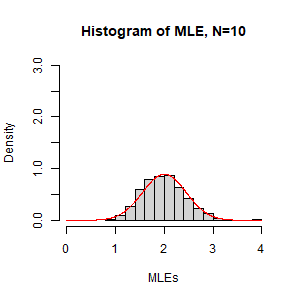
\includegraphics[scale=0.45]{../../../misc/N10.jpg}
    \end{subfigure}
    \begin{subfigure}
        \centering
        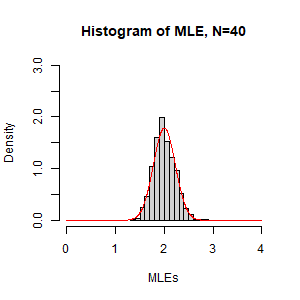
\includegraphics[scale=0.45]{../../../misc/N40.jpg}
    \end{subfigure}\\
    \begin{subfigure}
        \centering
        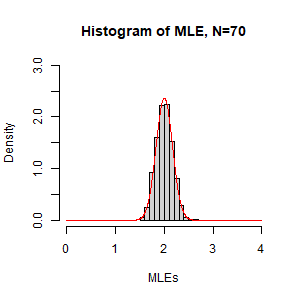
\includegraphics[scale=0.45]{../../../misc/N70.jpg}
    \end{subfigure}
    \begin{subfigure}
        \centering
        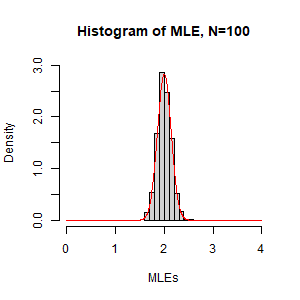
\includegraphics[scale=0.45]{../../../misc/N100.jpg}
    \end{subfigure}
	\caption{Histograms of MLEs of varying sample sizes}
	\label{hist}
\end{figure}
\subsection{Asymptotic Efficiency of MLE}
Having established \cref{thm:1}, it is natural to shift our attention to the quality of MLEs. The next result (\emph{Cramer-Rao lowerbound}) gives us some insight to the quality of MLEs compared to other estimators in terms of their variances. Note that by unbiased estimator, we mean estimators whose expectation is the true underlying parameter that is being estimated.
\begin{theorem}\label{thm:2}
Let $Y = u(X_1,\cdots,X_n)$ be an unbiased estimator of $\theta_0$ such that $\bbE_{\theta_0}[Y] = \theta_0$. Then under regularity conditions, $\var(Y) \geq \frac{1}{nI(\theta_0)}$.
\end{theorem}
\begin{proof}
We first expand $E_{\theta_0}[Y]$.
\begin{align*}
\theta_0 = E_{\theta_0}[Y] = \int_\bbR\cdots\int_\bbR u(x_1,\cdots,x_n)\prod_{i=1}^nf(x_i;\theta_0)dx_1\cdots dx_n.
\end{align*}
Differentiating both sides with respect to $\theta_0$ gives
\begin{align*}
1 &= \int_\bbR\cdots\int_\bbR u(x_1,\cdots,x_n) \left(\sum_{i=1}^n \frac{\partial f(x_i;\theta_0)}{\partial\theta_0} \frac{1}{f(x_i;\theta_0)}\right) \prod_{i=1}^nf(x_i;\theta_0)dx_1\cdots dx_n\\
&= \int_\bbR\cdots\int_\bbR u(x_1,\cdots,x_n) \left(\sum_{i=1}^n \frac{\partial \log f(x_i;\theta_0)}{\partial\theta_0} \right) \prod_{i=1}^nf(x_i;\theta_0)dx_1\cdots dx_n
\end{align*}
By writing $Z = \sum_{i=1}^n \frac{\partial \log f(X_i;\theta_0)}{\partial\theta_0}$, we get, with $\rho$ denoting the correlation coefficient between $Y$ and $Z$,
\begin{align*}
1 = \bbE_{\theta_0}[YZ] = \bbE_{\theta_0}[Y]\bbE_{\theta_0}[Z] + \rho\sqrt{\var(Y)}\sqrt{\var(Z)} \implies \rho = \frac{1}{\sqrt{\var(Y)}\sqrt{\var(Z)}}.
\end{align*}
We note that since $X_i$'s are \iid,
\begin{align*}
\var(Z) = \var\left( \sum_{i=1}^n \frac{\partial \log f(X_i;\theta_0)}{\partial\theta_0} \right)
= \sum_{i=1}^n \var\left(\frac{\partial \log f(X_i;\theta_0)}{\partial\theta_0}\right)
= n\var\left(\frac{\partial \log f(X_1;\theta_0)}{\partial\theta_0}\right)
= nI(\theta_0).
\end{align*}
Then $\rho = \frac{1}{\sqrt{nI(\theta_0)}\sqrt{\var(Y)}}$. By definition, $rho^2 \leq 1$, then
\begin{align*}
\rho^2 = \frac{1}{nI(\theta_0)\var(Y)} \leq 1 \implies \var(Y) \geq \frac{1}{nI(\theta_0)}.
\end{align*}
Therefore for any unbiased estimator $Y$ of $\theta_0$, we have $\var(Y) \geq \frac{1}{nI(\theta_0)}$.
\end{proof}
$ $\\
The proof itself is relatively straightforward, where we essentially reach the desired conclusion by using (R5) of the regularity conditions and simple algebraic manipulations. It is, however, the implication of this result that is worth looking at. Note the lower bound on the variance is exactly the asymptotic variance of MLEs. This means that asymptotically, the MLE achieves the smallest possible variance out of all unbiased estimators of $\theta$. Therefore the MLEs are said to be \emph{asymptotically efficient}.\\\\
While this is a nice property, it remains rather theoretical. In practice, when we work with finitely many observations, it is not clear how far away we are from the asymptotic normality. And existing heuristics from undergraduate statistics courses such as calling samples larger than $25$ or $30$ large enough is far from satisfying. Fortunately, \cite{anastasiou2015bounds} have done some pioneer work aimed at answering this exact question. We turn in the next section for a brief illustration of their result on the the closeness from the MLE approximated using finitely many observations to the asymptotic normal distribution.
% ...